In this part of the study, how the quantitative measurement methods are applied and these measurements' results are discussed. Besides, the findings obtained from the comparison of the results are also shared in this section.

\subsubsection{Sample Codebases}
\label{section:5.3.1}
Before moving on to the results and comparisons of quantitative measurement methods, it will be useful to understand how and under what conditions these methods are applied to understand the results better. Previously quantitative measurement methods, metrics to be used and information on why they were chosen shared in section \ref{section:3.2}. More detailed information about the codebases to which these metrics were applied and why these codebases were selected will be shared in this subsection.

As mentioned in section \ref{section:3.2}, two codebases belonging to the same project have been selected to apply the metrics. The first of these codebases, defined as \textbf{\textit{cb-1}} in this study, represents the unorganized codebase that has been poorly structured. The second of these codebases is a well-structured code base, which has been defined as \textbf{\textit{cb-2}} and started to be developed using the technologies and methods mentioned in detail in section \ref{section:2.3}. To facilitate the explanation, these codebases will be mentioned in the form of \textbf{\textit{cb-1}} and \textbf{\textit{cb-2}} in the remainder of the study.

When cb-1 is examined in detail, a situation like the following is encountered. First of all, the Android application's active version implemented with this project is working on this codebase, and it is actively used. The project was started to be developed using the Java programming language. Later, some features were developed using Kotlin programming language. There is no consistent choice of software architecture throughout the application. Although the application consists of 5 different modules, the modules' boundaries are not determined according to a certain standard. Some modules are feature-based, while some are layer-based. A similar situation is observed in packaging. The packaging organization of the application is inferior. While some features of the application have been developed with the MVP design pattern, some features have been developed with MVVM. It is controversial to what extent these design patterns are applied correctly. Static classes and singleton solutions have been used dangerously in practice. Besides, the SOLID principles have been partially ignored, while the dependency injection principles have been completely ignored. It is also worth noting the use of several outdated libraries. Finally, some low-maintainability manual solutions have been used for networking and database spaces. Also, when looking at the Git history of the application, the commits of 11 different developers are seen. This situation is critical in describing the developer circulation in the application and explaining its serious organisation problems. The relationship between the developer circulation and the maintainability of software systems was previously mentioned in section \ref{section:1.1}. Considering the date this application started to be developed, the use of old-fashioned technologies is normal, but the lack of organization throughout the application is unusual. This unusual situation and the other features listed above seriously affect the understandability and maintainability of the application. On the other hand, this situation offers a great opportunity for this study to measure maintainability.

When looking at cb-2, it is seen that the opposite of cb-1 is the case. It was decided to develop this version of the application because the problems in cb-1 became more visible, and the maintainability problems increased. While this version of the application is being developed, methods, technologies and architecture, detailed in section \ref{section:2.3}, were used. It has started to be developed using Kotlin programming language, and the entire application is in Kotlin programming language.  Clean architecture and clean code, and SOLID principles are followed during the development. The application modules are separated based on the layers, and the packaging is feature-based. While developing the application, maintainable and reliable Android libraries have been used. The organisation level of the application's this version is very high, and it has been arranged to be a standard throughout the whole application. On the other hand,  development for this version of the application's is still ongoing, and there are only 4 main features that have already been developed. The features currently developed for cb-2 are splash, login, register and main screen features. In this respect, cb-2 falls short in terms of fully developed features compared to cb-1.

The following section explains how both of these codebases were used while conducting the quantitative evaluation.




\subsubsection{CodeMR}
The CodeMR tool uses different visualization methods in the reports generated by the application of metrics. The charts are created with the help of these different visualization techniques based on the metric values obtained from the analysis conducted by the tool. In this study, the visualization methods known as "Metric Distribution" and "Package Structure" were preferred to present the results of the evaluations. The main reason for choosing this methods is that it makes the visual understanding of the results easier than other methods and also these methods provide a better situational perceptibility for projects. These visualization techniques were used to visualize the data obtained as a result of applying the metrics specified in section 3.2 and the analysis presented by CodeMR on complexity, coupling and cohesion concepts. Other visualization methods and charts are very detailed, and sharing such detailed results is beyond this study's scope. The tool also presents the values for each metric over the provided codebase and presents these values. Values for each metric are presented at project, module, package and class scopes. However, in the evaluations within the scope of this study, only the results of the metrics previously determined and explained in section \ref{section:4.2} were used and these metrics are Weighted Method
Count (WMC), Depth of Inheritance Tree (DIT), Number of Children (NOC), Coupling Between Object Classes (CBO), and Lack of Cohesion of Methods (LCOM). Fig \ref{fig:code-mr-metric-val} presents the metric values calculated with the help of the CodeMR Intellij IDEA plugin.
\begin{figure}[ht!]
    \centering
    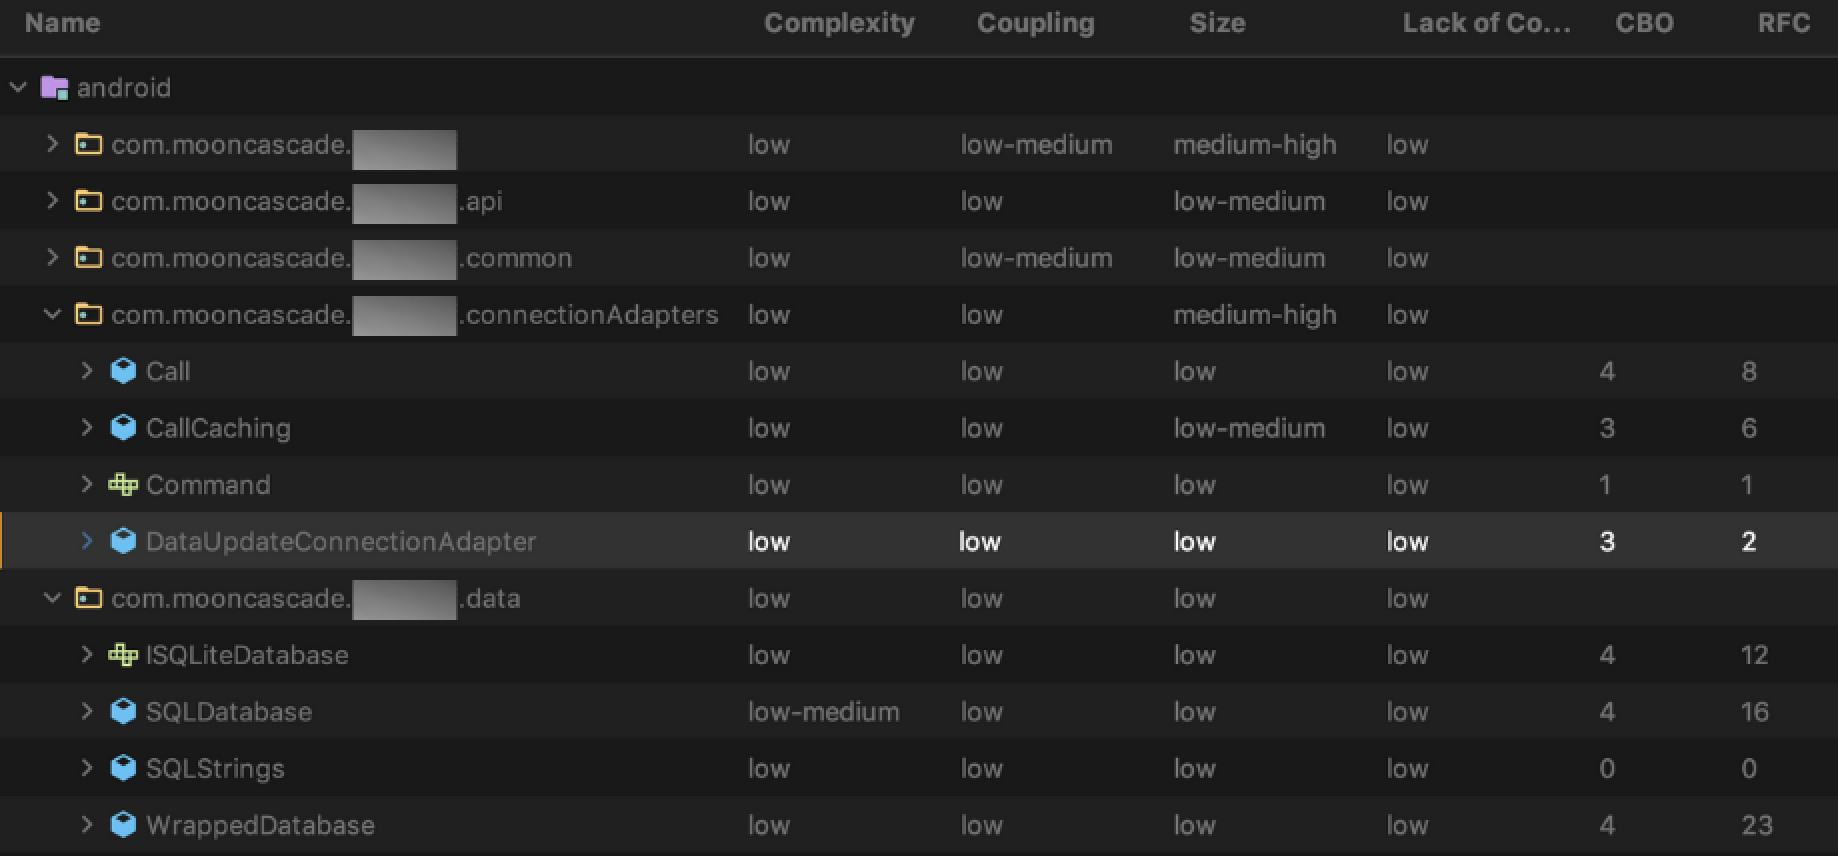
\includegraphics[scale=0.35]{figures/code-mr-metric-val.png}
    \caption{CodeMR Metric Value Presentation}
    \label{fig:code-mr-metric-val}
\end{figure}
\FloatBarrier

There are two important points to be aware of when interpreting the charts created by these methods using CodeMR. The first of these points is legends used to indicate metric levels. As can be seen in Fig. \ref{fig:code-mr-legends}, each colour corresponds to a metric level that is represented by a certain metric value threshold. For the metrics selected for this study, low values tend to indicate better results while high values point to the contrary.
\begin{figure}[ht!]
    \centering
    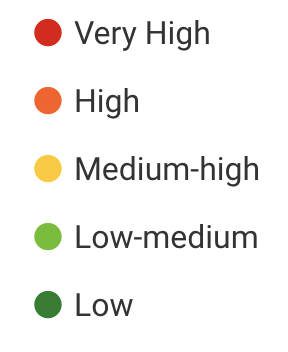
\includegraphics[scale=0.7]{figures/code-mr-legends.png}
    \caption{CodeMR Metric Level Indicators}
    \label{fig:code-mr-legends}
\end{figure}
\FloatBarrier

The second important point is how the percentages on these charts are calculated while realizing the charts created by CodeMR. There might be different metric levels in different percentages in the charts. These percentages of metric levels for the selected metrics are illustrated in charts proportionally to the code size of classes in this level. Detailed information about the formulas used in calculating metric values and how the values are interpreted amd visualized can be accessed through the CodeMR documentation\footnote{\label{fn:codemr} \url{https://www.codemr.co.uk/documents/}}.

Presentation of the results obtained via CodeMR is done as explained below. The charts and the  metrics values obtained from the evaluation are shared. Although these techniques can be applied at the class and package level, it was preferred to present the project level results. It would not be very effective and useful to present these results for each class and package since there are many classes and packages for both codebases. On the other hand, at the class level, for making some evaluation and comparison, a few sample classes with high functionality were selected from both codebases, and they were evaluated and compared. Also, in accordance with the confidentiality requirements, the package and class names that will call the application name were hidden in the shared analysis results and figures. Then the results were presented via visualisation methods and numeric values. Following sections present the evaluation results and findings.

%$^{\ref{fn:codemr}}$.



\subsubsection{Way of Evaluation and Presentation of Results}
The details of the metrics selected for quantitative evaluations and that these metrics will be applied on codebases using the CodeMR static code analysis tool are mentioned in section \ref{section:3.2}. However, the information that would facilitate the interpretation of the charts and reports produced by CodeMR was not shared. It is deemed appropriate to share this information in this section so that the results can be understood and interpreted more easily.

The CodeMR tool uses different visualization methods in the reports generated by the application of metrics. The details of these visualization methods and the types of charts used are detailed in the CodeMR documentation \footnote{ \url{https://www.codemr.co.uk/documents/}}. Within this study's scope, the visualization method known as "Metric Distribution" in CodeMR literature and presenting the results in the form of a pie chart was preferred. The main reason for choosing this method is that it makes the visual understanding of the results easier than other methods. Other visualization methods and charts are very detailed, and sharing such detailed results is beyond this study's scope. There are two important points to be aware of when interpreting pie charts created by the "Metric Distribution" method using CodeMR. The first of these points is legends used to indicate metric levels. As can be seeń in Fig. \ref{fig:code-mr-legends}, each colour corresponds to a metric level.
\begin{figure}[ht!]
    \centering
    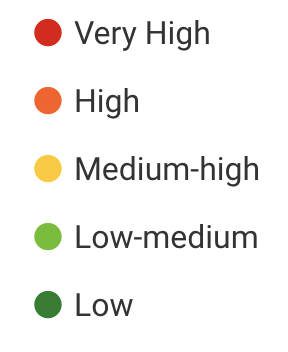
\includegraphics[scale=0.7]{figures/code-mr-legends.png}
    \caption{CodeMR Metric Level Indicators}
    \label{fig:code-mr-legends}
\end{figure}

The second important point is how the percentages on these graphs are calculated while realizing the pie charts created by CodeMR. Below is a pie chart created by CodeMR using the "Metric Distribution" method and the "Size" sample metric.
\begin{figure}[ht!]
    \centering
    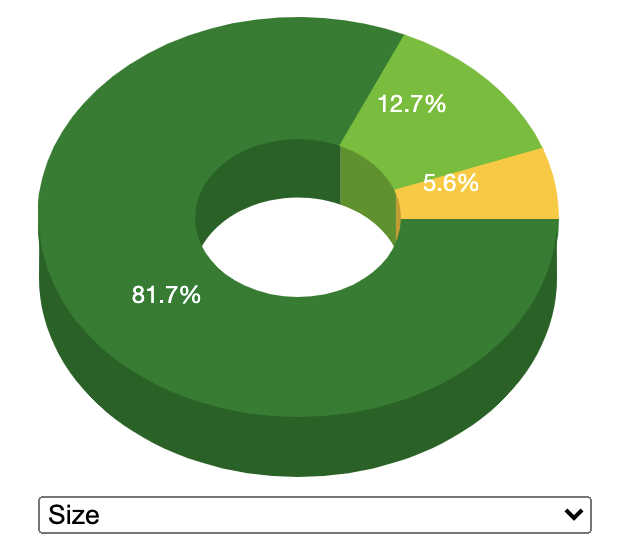
\includegraphics[scale=0.6]{figures/sample-code-mr-chart.png}
    \caption{Sample CodeMR Pie Chart}
    \label{fig:sample-code-mr-chart}
\end{figure}
\FloatBarrier

As can be seen in Fig. \ref{fig:sample-code-mr-chart}, there are 3 different metric levels in different percentages in the graph. These percentages of metric levels for the selected metric are illustrated in a pie chart proportional to the code size of classes in this level. In other words, the slices of pie charts are proportional to the code volume of classes for the corresponding level.

As explained above, these two points are essential when interpreting pie charts that will be shared in the next three sections. In the following sections, the results of this evaluation and the findings for comparisons are shared.



\subsubsection{CB-1 Results}
When the numerical analysis results performed on the cb-1 via the CodeMR tool are examined, it is seen that the tool analyzes 2079 lines of code belonging to this codebase. These lines of code belong to 118 classes in 12 different packages of 4 different features which were mentioned in section \ref{section:5.3.1}. When the metric values of the analysis result performed by the CodeMR tool of the cb-1 are reviewed, some problems draw attention, although the general situation is not extremely problematic. In the figure below, a CodeMR table that reflects the general situation of cb-1 is shared. In this table, a grouped overview of the complexity, coupling and cohesion levels determined through the metric values obtained from the analysis of the codebase is shown.
\begin{figure}[ht!]
    \centering
    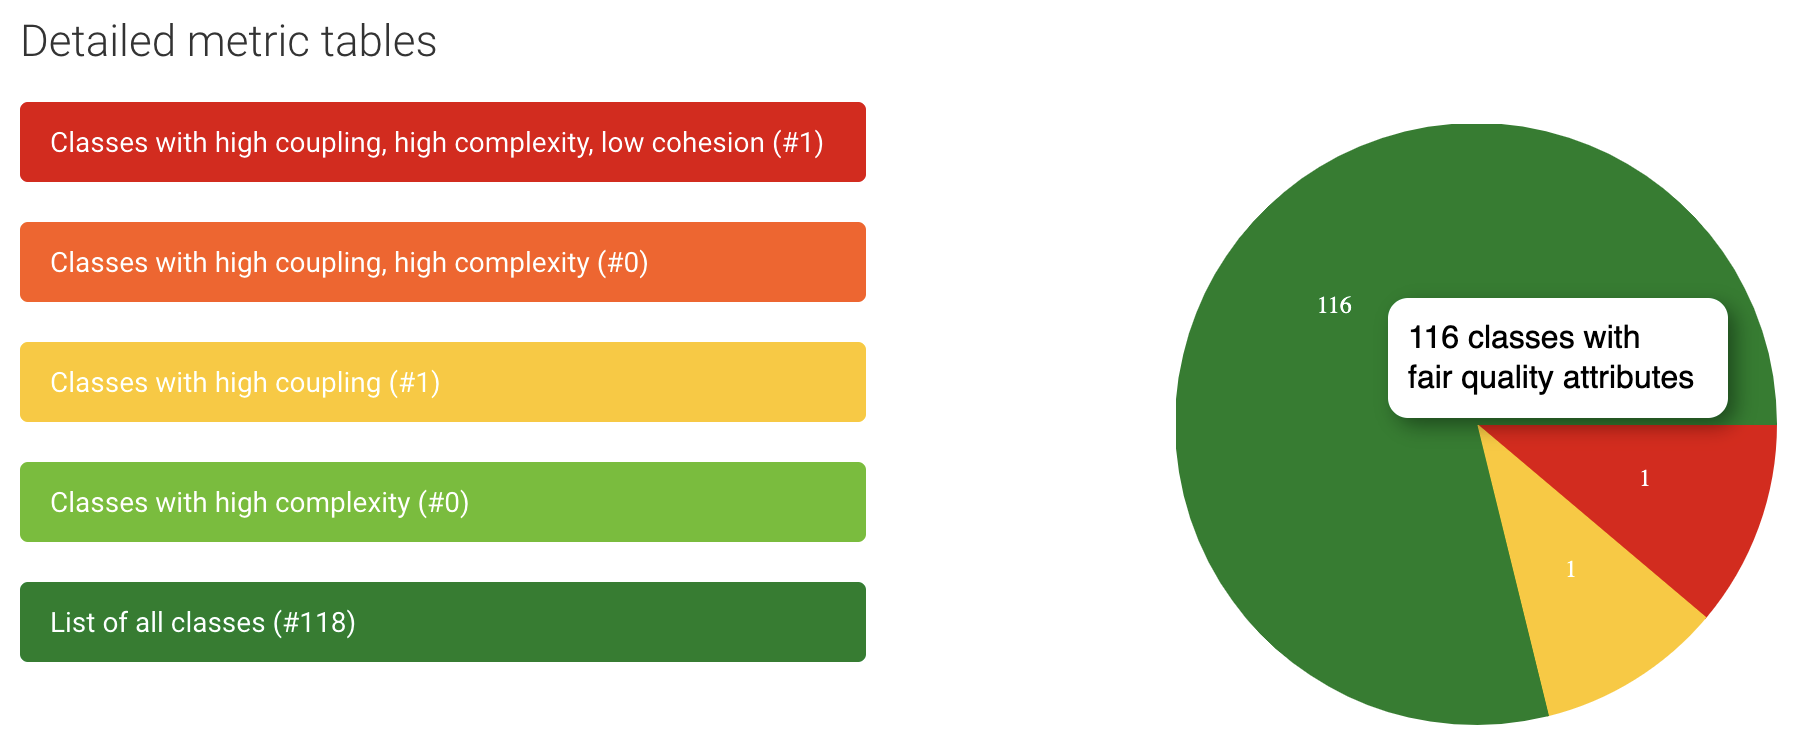
\includegraphics[scale=0.45]{figures/cb-1-metric-table.png}
    \caption{CodeMR Metrics Overview of CB-1}
    \label{fig:cb-1-metric-table.png}
\end{figure}
\FloatBarrier
The detailed evaluation of the results on the basis of metric is as follows. Among the analyzed classes, it is seen that two classes corresponding to 23\% of the total code size have medium-high WMC values. It is seen that these classes, which are classified as A and B classes, have WMC values of 61 and 58, respectively. There are also two other classes corresponding to 14\% code size have low-medium WMC values. Rest of the classes appear to have low level of WMC values.  When the values of the DIT metric of the classes are examined, it is seen that 14 classes, corresponding to 22.7\% of the total code size, have middle-upper level DIT values and the other 14 classes corresponding to 26.4\% of the total code size have low-medium level DIT values. When the NOC metric values of the classes are examined, it is seen that 7 classes corresponding to only 3.4\% of the whole codebase have low-medium NOC values and all other classes have low NOC values. According to the results, it is seen that a class, which corresponds to 12.5\% of the code volume of the application, has a very high COB value. It also appears that a class that is corresponding to 11.2\% of the application's code volume has a high COB value, and another class that is corresponding to 4.4\% of the code volume has a medium-high COB value. When the values of LCOM, the last of the selected metrics, are examined on a class basis, it is seen that 6 classes corresponding to 40.8\% of the total code size have high LCOM values. Besides, it is seen that two classes have middle-upper level LCOM values, which corresponds to approximately 4\% of the total code size. In the figure below, the results of the class-based metric values, which is detailed and interpreted above, visualized by the "Metric Distribution" method offered by the CodeMR tool are presented. Charts are in doughnut form, and information regarding the methods of creating them has been shared in the previous sections. As previously mentioned,  the size/percentage of each part in the doughnut is proportional to the size of the class/interface it represents. The detailed interpretation of the data shared in the figure below and the metric values obtained from the analysis is made in section \ref{section:6.3.1}.

\begin{figure}[ht!]
    \centering
    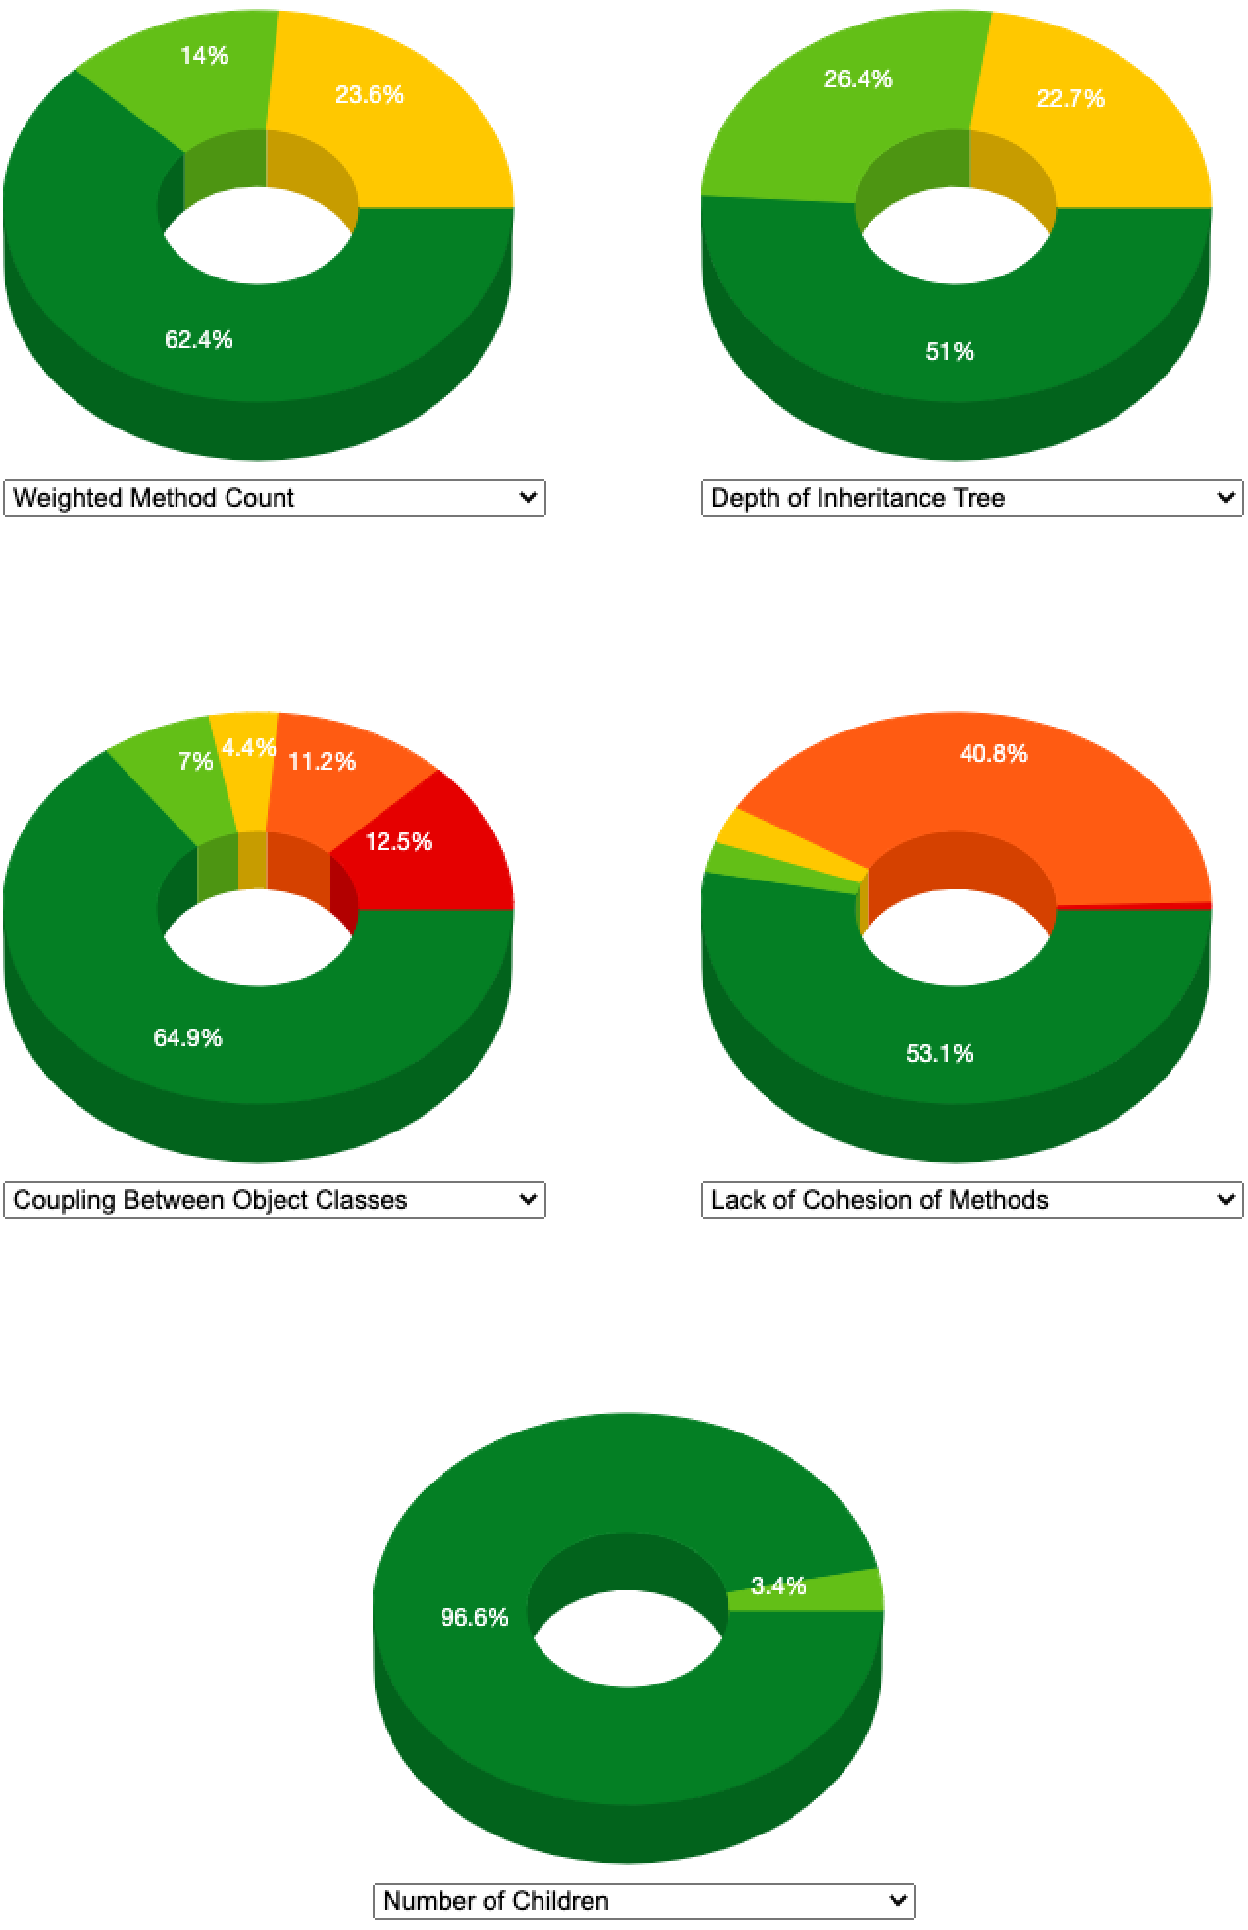
\includegraphics[scale=1]{figures/cb-1-donuts.png}
    \caption{CodeMR Metric Distribution for CB-1}
    \label{fig:cb-1-donuts}
\end{figure}
\FloatBarrier

In the figure below, a more general view of cb-1 in terms of complexity, coupling and cohesion is presented. In Fig. \ref{fig:cb-1-package}, the largest circle represents the project, while the inner circles represent the packages and the small circles inside the inner circles represent the classes. The size of each circle is directly proportional to the size of the structure it represents. The detailed interpretation of the  the figure below is made in section \ref{section:6.3.1}.

\begin{figure}[ht!]
    \centering
    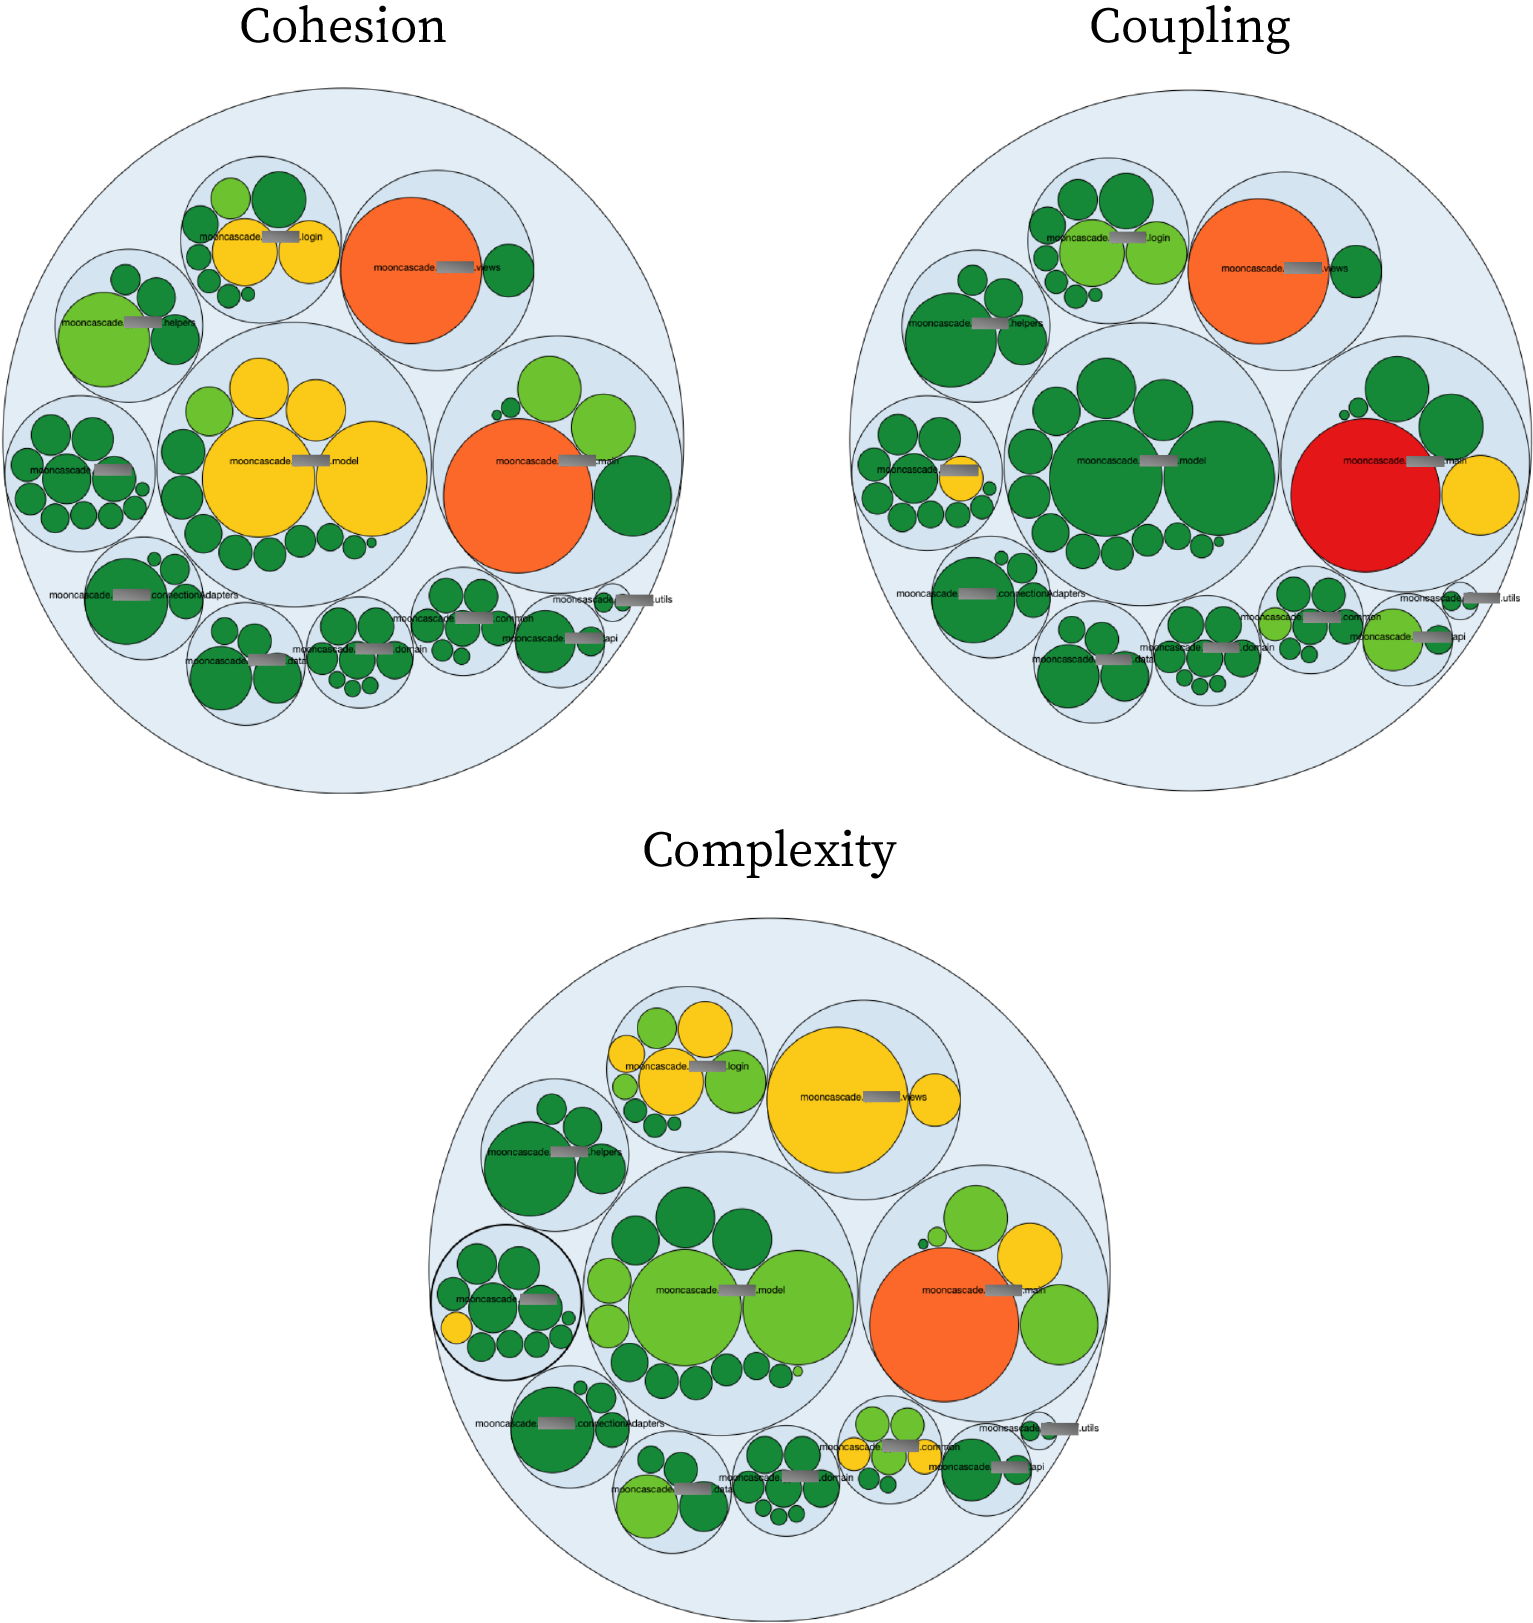
\includegraphics[scale=1.1]{figures/cb-1-package.png}
    \caption{CodeMR Metric Values by Packages for CB-1}
    \label{fig:cb-1-package}
\end{figure}
\FloatBarrier



\subsubsection{CB-2 Results}
When the numerical analysis results produced on the cb-2 via the CodeMR tool are reviewed, it is seen that the tool analyzes 1160 lines of code belonging to this codebase. These lines of code belong to 139 classes in 59 different packages of 4 different features which were mentioned in section \ref{section:5.3.1}. When the CodeMR analysis results of this codebase are examined, a very positive situation is encountered. In the figure below, a CodeMR table that reflects the general situation of cb-2 is shared.
\begin{figure}[ht!]
    \centering
    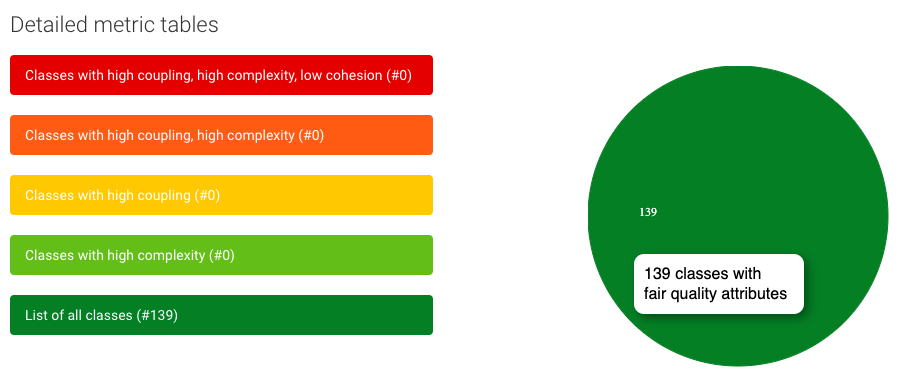
\includegraphics[scale=0.45]{figures/cb-2-metric-table.png}
    \caption{CodeMR Metrics Overview of CB-2}
    \label{fig:cb-2-metric-table.png}
\end{figure}
\FloatBarrier

Between the analyzed classes, it is seen that two classes corresponding to 9\% of the total code size have low-medium WMC values, and the rest of the classes appear to have a low level of WMC values. It appears that the majority of the classes belong to cb-2 have low complexity levels. When the values of the DIT metric of the classes are examined, it is seen that 10 classes, corresponding to 28.9\% of the total code size, have middle-upper level DIT values and the other 27 classes corresponding to 14.1\% of the total code size have low-medium level DIT values. The rest of the classes have a low level of DIT values.  When DIT values of these classes are examined, it is seen that some classes have a DIT value of 2 and classes with more than a DIT value of 2 values are quite low (DIT values between 1-3 considered as low-medium by CodeMR). When the NOC metric values of the classes are examined, it is seen that 7 classes corresponding to only 6.6\% of the whole codebase have low-medium NOC values, and 1 very concise class has medium-high NOC value. The rest of the classes have low NOC values. According to the results, it is seen that ten classes are corresponding to 26.6\% of the application's code volume with a low-medium COB value and the rest of the classes have a low COB value. According to the results of the CodeMR analysis, all classes within the cb-2 have low LCOM values. According to the results of the CodeMR analysis, all classes within the cb-2 have low LCOM values. In the figure below, the results of the class-based metric values, which is detailed and interpreted above, visualized by the "Metric Distribution" method offered by the CodeMR tool are presented. The detailed interpretation of the data shared in the figure below and the metric values obtained from the analysis is made in section \ref{section:6.3.2}.

\begin{figure}[ht!]
    \centering
    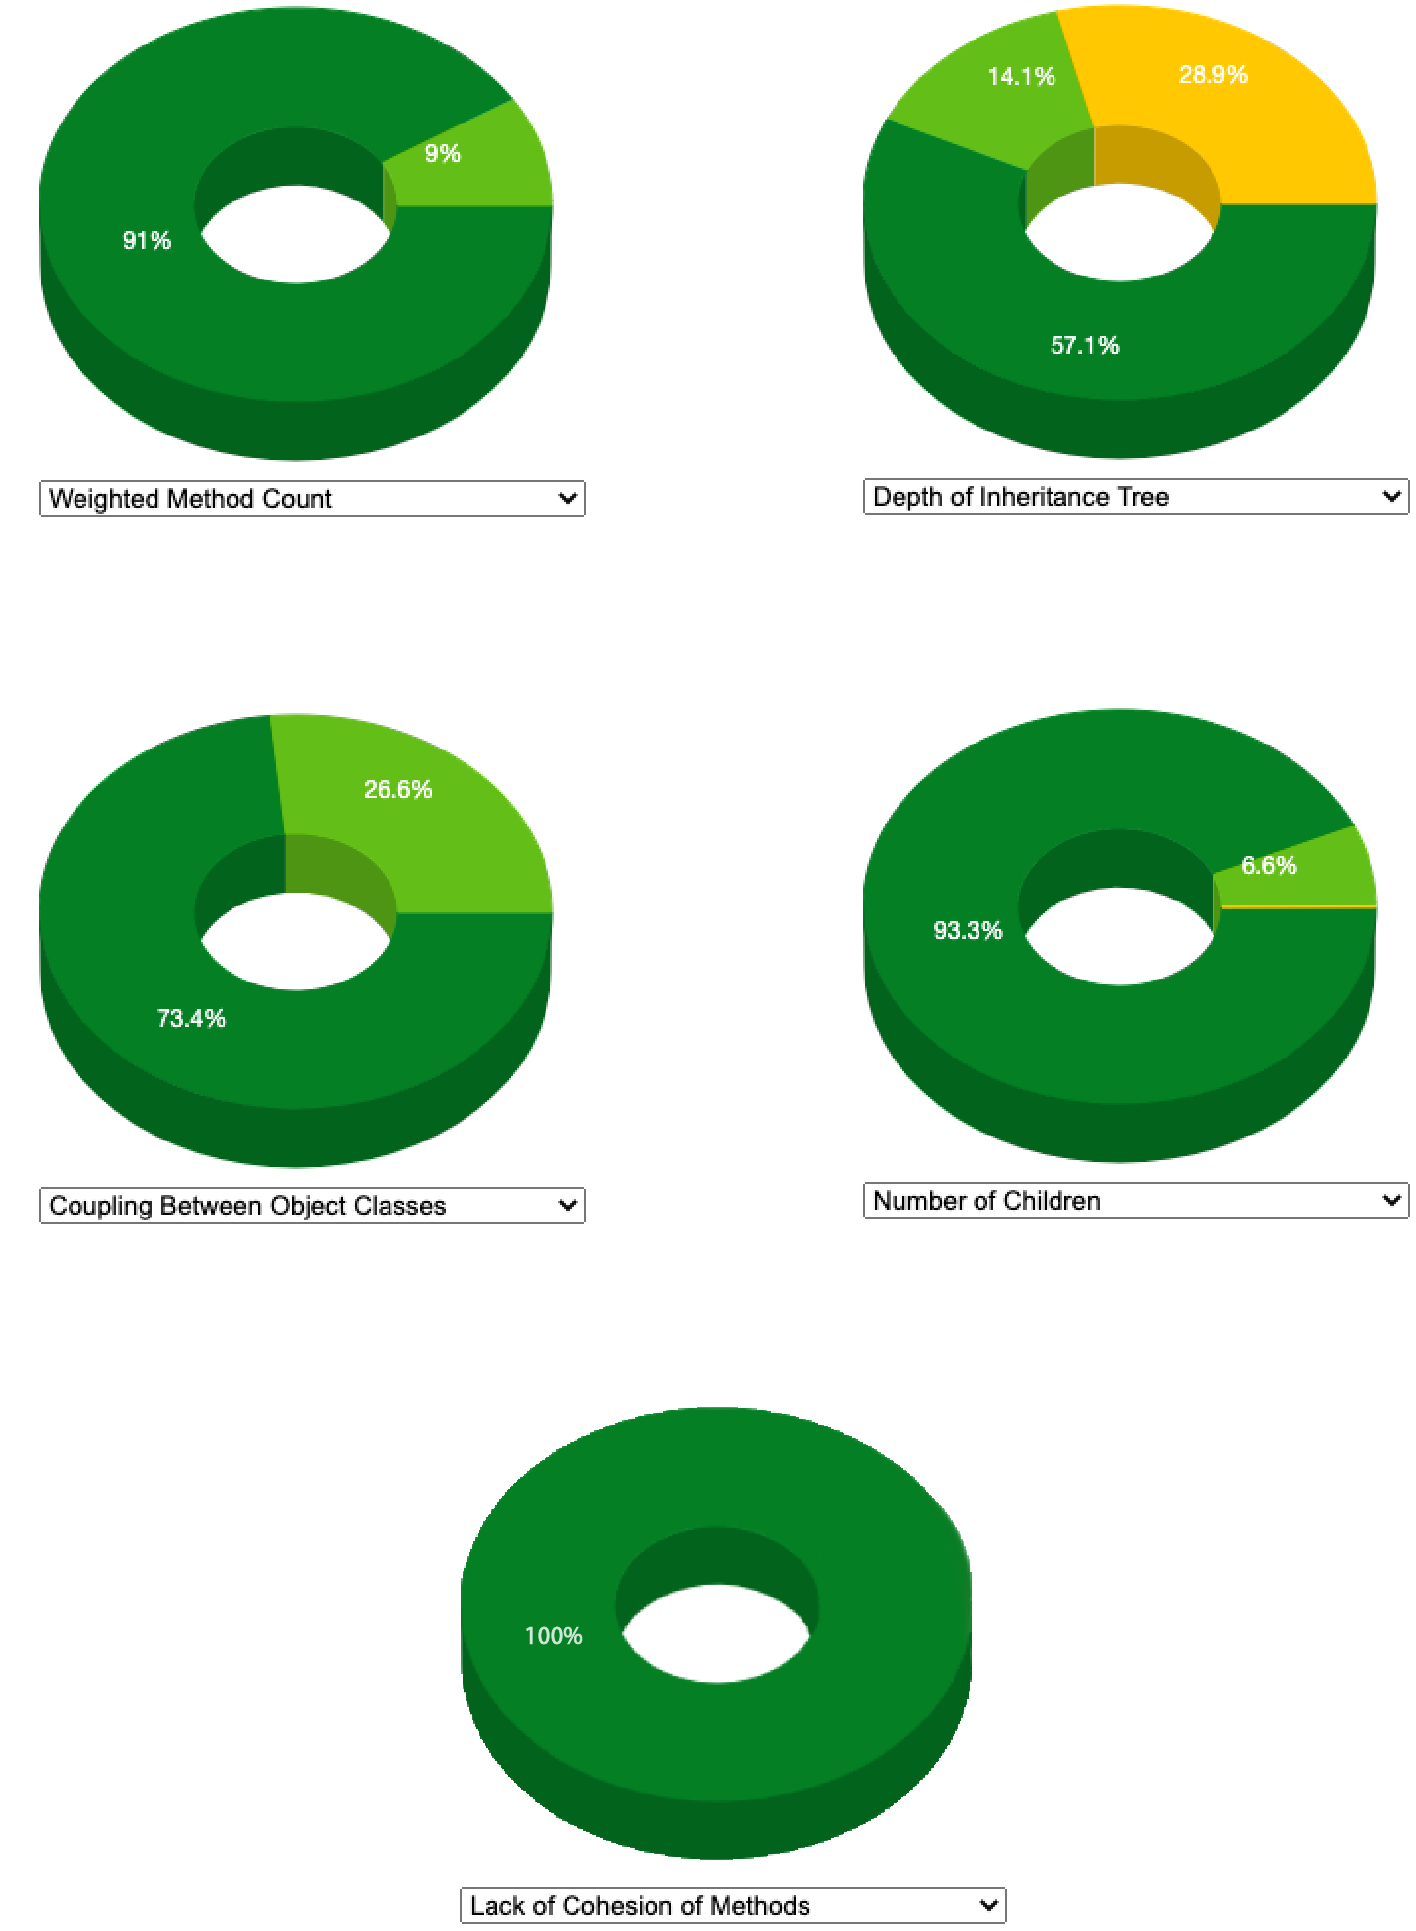
\includegraphics[scale=1]{figures/cb-2-donuts.png}
    \caption{CodeMR Metric Distribution for CB-2}
    \label{fig:cb-2-donuts}
\end{figure}
\FloatBarrier

In the figure below, a general view of cb-2 in terms of complexity, coupling and cohesion is shown. As explained in the previous section, the largest circle represents the project, inner circles represent the packages and small circles inside the inner circles represent the classes. Sizes of the circles proportional to the size of the represented entity. The detailed interpretation of the figure is made in section \ref{section:6.3.2}.
\begin{figure}[ht!]
    \centering
    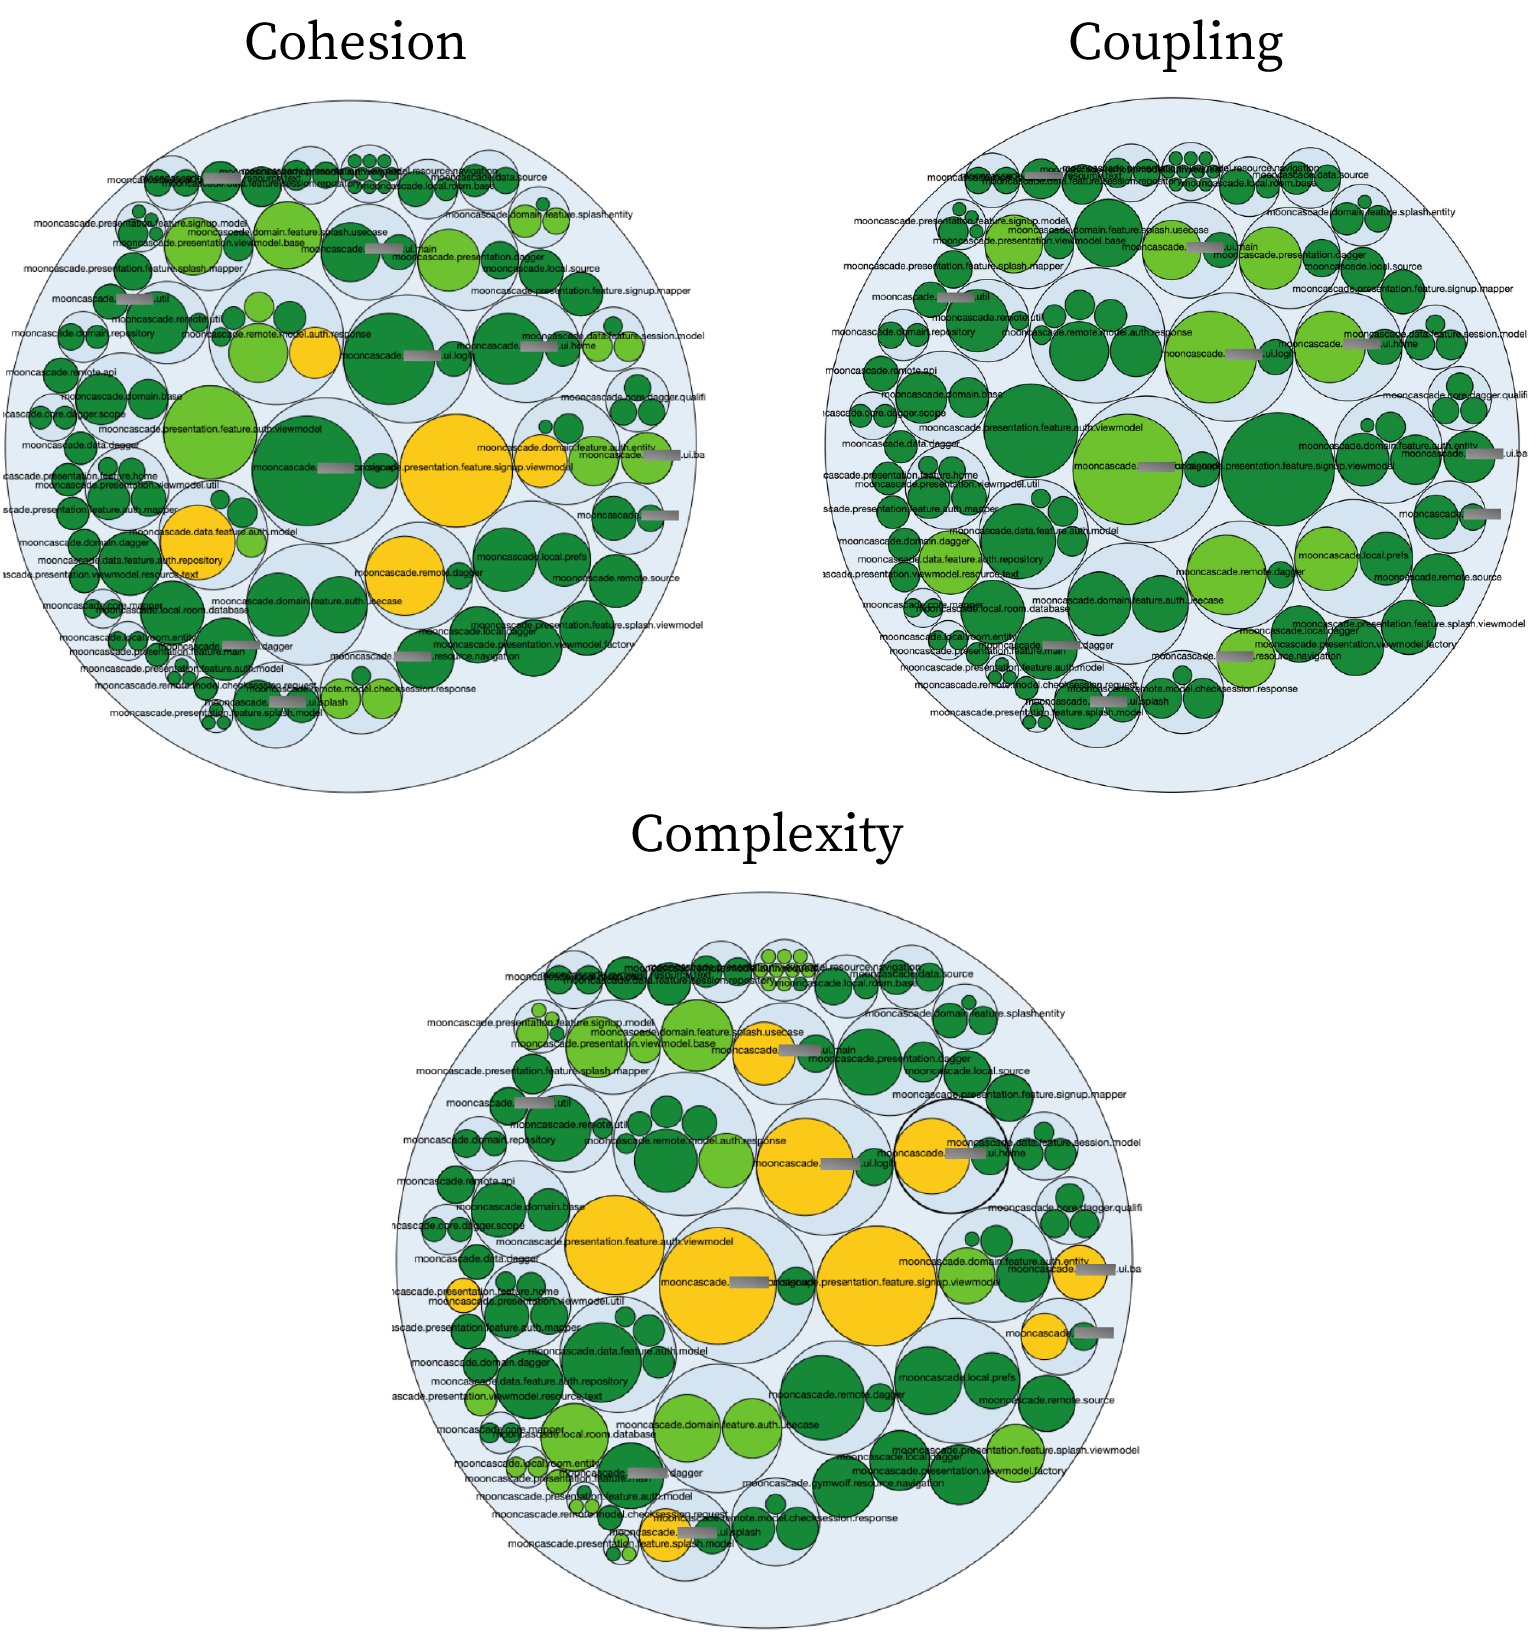
\includegraphics[scale=1.1]{figures/cb-2-package.png}
    \caption{CodeMR Metric Distribution for CB-2}
    \label{fig:cb-2-package}
\end{figure}
\FloatBarrier







\subsubsection{Feature-Based Comparison Results}
In this section, results obtained from comparing the analysis of cb-1 and cb-2 codebases are shared. The analysis results of the two codebases have been compared to make a more efficient evaluation. Besides, to make a more effective evaluation, the numerical evaluation results obtained from a few sample classes with high functionality were collected, and the results were compared. To get more accurate results, while selecting the sample classes, classes with high complexity and more detailed business logic were studied. Evaluations of all these comparisons are shared in this section.

The login feature has been selected from among the available features to compare the maintainability differences between the two codebases. The reason for choosing it is that it has a more complex logic (e.g. validation, different error types, etc.) than other existing features mentioned in the previous sections. Classes containing view and view logic parts for the login feature from both codebases have been selected for comparison. While making the evaluation, other lower-level dependencies were excluded. When the cb-1 using the MVP design pattern is examined, it is seen that 6 classes and interfaces are used related to the presentation and logic of data related to login. These classes and interfaces are: LoginActivityView (interface), LoginActivity (class), LoginActivityPresenter (class), LoginFragmentView (interface), LoginFragment (class), LoginFragmentPresenter (class). When the cb-2, which uses the MVVM design pattern, is examined, it is seen that only 2 classes are used and they are LoginActivity and LoginViewModel. The difference in the number of classes and interfaces used for the login feature in the codebases is due to the differences in the design patterns used and the fact that the cb-1 also uses the Fragment class of Android. In Fig. \ref{fig:login-metric-table}, the metric values of each class listed above, obtained from the quantitative evaluation results, can be seen in the form of a table. The metric values shared in the tables were obtained as a result of the analysis performed using the Android Studio CodeMR plugin.
\begin{figure}[ht!]
    \centering
    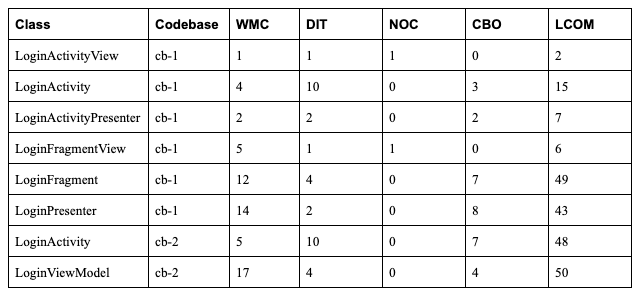
\includegraphics[scale=0.65]{figures/login-metric-table.png}
    \caption{CodeMR Metric Values for Login Feature}
    \label{fig:login-metric-table}
\end{figure}
\FloatBarrier

In order to examine the results better, groupings can be made between these classes, and the metric values of these groups can be compared. This grouping can be made based on the responsibilities of the classes. The responsibilities to be taken as a basis while groups are determined as view and view logic. More detailed information on these responsibilities was shared in previous sections. These classes and their interfaces can be grouped for each codebase as follows. For cb-1, LoginActivityView, LoginActivity, LoginFragmentView and LoginFragment are only responsible for the presentation of the data.  LoginActivityPresenter and LoginFragmentPresenter are the classes responsible for how and when the data is presented. For cb-2, LoginActivity is responsible for presenting data, and LoginViewModel is responsible for how and when data is presented. This grouping will be useful for comparing the metric values shared in Fig. \ref{fig:code-mr-metric-val}. In the table below, the metric values for each group of both codebases that are obtained from the analysis made within the scope of this study are shared.

\begin{figure}[ht!]
    \centering
    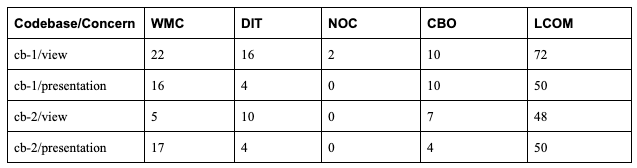
\includegraphics[scale=0.65]{figures/login-metric-table-2.png}
    \caption{CodeMR Metric Values for Login Feature}
    \label{fig:login-metric-table-2}
\end{figure}
\FloatBarrier

Although the interpretation of the results is partially possible when the data in the above-shared tables are examined, the interpretation and detailed analysis of this given are made and shared in section \ref{section:6.3.5}.
